%%%%%%%%%%%%%%%%%%%%%%%%%%%%%%%%%%%%%%%%%
% Beamer Presentation
% LaTeX Template
% Version 1.0 (10/11/12)
%
% This template has been downloaded from:
% http://www.LaTeXTemplates.com
%
% License:
% CC BY-NC-SA 3.0 (http://creativecommons.org/licenses/by-nc-sa/3.0/)
%
%%%%%%%%%%%%%%%%%%%%%%%%%%%%%%%%%%%%%%%%%

%----------------------------------------------------------------------------------------
%	PACKAGES AND THEMES
%----------------------------------------------------------------------------------------

\documentclass[fleqn]{beamer}

\mode<presentation> {

% The Beamer class comes with a number of default slide themes
% which change the colors and layouts of slides. Below this is a list
% of all the themes, uncomment each in turn to see what they look like.

%\usetheme{default}
%\usetheme{AnnArbor}
%\usetheme{Antibes}
%\usetheme{Bergen}
%\usetheme{Berkeley}
%\usetheme{Berlin}
%\usetheme{Boadilla}
%\usetheme{CambridgeUS}
%\usetheme{Copenhagen}
\usetheme{Darmstadt}
%\usetheme{Dresden}
%\usetheme{Frankfurt}
%\usetheme{Goettingen}
%\usetheme{Hannover}
%\usetheme{Ilmenau}
%\usetheme{JuanLesPins}
%\usetheme{Luebeck}
%\usetheme{Madrid}
%*\usetheme{Malmoe}
%\usetheme{Marburg}
%\usetheme{Montpellier}
%\usetheme{PaloAlto}
%\usetheme{Pittsburgh}
%\usetheme{Rochester}
%\usetheme{Singapore}
%\usetheme{Szeged}
%\usetheme{Warsaw}

% As well as themes, the Beamer class has a number of color themes
% for any slide theme. Uncomment each of these in turn to see how it
% changes the colors of your current slide theme.

%\usecolortheme{albatross}
%\usecolortheme{beaver}
%\usecolortheme{beetle}
%\usecolortheme{crane}
%\usecolortheme{dolphin}
%\usecolortheme{dove}
%\usecolortheme{fly}
%\usecolortheme{lily}
\usecolortheme{orchid}
%\usecolortheme{rose}
%\usecolortheme{seagull}
%\usecolortheme{seahorse}
%\usecolortheme{whale}
%\usecolortheme{wolverine}

%\setbeamertemplate{footline} % To remove the footer line in all slides uncomment this line
%\setbeamertemplate{footline}[page number] % To replace the footer line in all slides with a simple slide count uncomment this line

%\setbeamertemplate{navigation symbols}{} % To remove the navigation symbols from the bottom of all slides uncomment this line
}


\usepackage{graphicx} % Allows including images
\usepackage{booktabs} % Allows the use of \toprule, \midrule and \bottomrule in tables
\usepackage{xspace}
\usepackage{caption}
\usepackage{subfigure}
\usepackage[english,brazil]{babel}
\usepackage[utf8]{inputenc}

%Renomeia o nome padrao das figuras.
\renewcommand{\figurename}{Figura}
\renewcommand{\tablename}{Tabela}
%----------------------------------------------------------------------------------------
%	TITLE PAGE
%----------------------------------------------------------------------------------------

\title[Computação Gráfica]{Transformações 2D} % The short title appears at the bottom of every slide, the full title is only on the title page

\author{Uéliton Freitas} % Your name
\institute[UFMS] % Your institution as it will appear on the bottom of every slide, may be shorthand to save space
{
Universidade Católica Don Bosco - UCDB \\ % Your institution for the title page
\medskip
\textit{freitas.ueliton@gmail.com} % Your email address
}
\date{\today} % Date, can be changed to a custom date


\begin{document}

\begin{frame}
\titlepage % Print the title page as the first slide
\end{frame}

\begin{frame}
\frametitle{Sumário} % Table of contents slide, comment this block out to remove it
\tableofcontents % Throughout your presentation, if you choose to use \section{} and \subsection{} commands, these will automatically be printed on this slide as an overview of your presentation
\end{frame}




%----------------------------------------------------------------------------------------
%	PRESENTATION SLIDES
%----------------------------------------------------------------------------------------

%------------------------------------------------
\section{Introdução} 
%------------------------------------------------

%\section{Speeded-Up Robust Features - SURF} % A subsection can be created just before a set of slides with a common theme to further break down your presentation into chunks
%\section{Baf Of Features and Colors}

%\section{Refer\^encias}
%%%%%%%%%%%%%%%%%%%%%%%%%%%%%%%%%%%%%%%%%%%%%%%%%%%%%%%%%%%%%%%%%%%%%%%%%%%%%%%%%%%%%%%%%%
\begin{frame}
\frametitle{Introdução}


	\begin{block}{Transformações Geométricas}
		\begin{itemize}
			\item São transformações aplicadas aos modelos de objetos:
				\begin{itemize}
					\item Posicionamento (translação).
					\item Orientação (rotação). 
					\item Tamanho (escala).
					\item Reflexão.
					\item Crisalhamento.
				\end{itemize}
		\end{itemize}
	\end{block}
	
\end{frame}

%%%%%%%%%%%%%%%%%%%%%%%%%%%%%%%%%%%%%%%%%%%%%%%%%%%%%%%%%%%%%%%%%%%%%%%%%%%%%%%%%%%%%%%%%%
\section{Translação}
\begin{frame}
\frametitle{Translação}


	\begin{block}{Translação de um Objeto}
		\begin{itemize}
			\item A translação consiste em adicionar uma ``variação'' as coordenadas de um objeto.
			\begin{itemize}
				\item $x' = x + \Delta x$
				\item $y' = y + \Delta y$
			\end{itemize}
		\end{itemize}
		
	\end{block}
	
\end{frame}

%%%%%%%%%%%%%%%%%%%%%%%%%%%%%%%%%%%%%%%%%%%%%%%%%%%%%%%%%%%%%%%%%%%%%%%%%%%%%%%%%%%%%%%%%%

\begin{frame}
\frametitle{Translação}
	\begin{figure}[!h]
			\begin{center}
			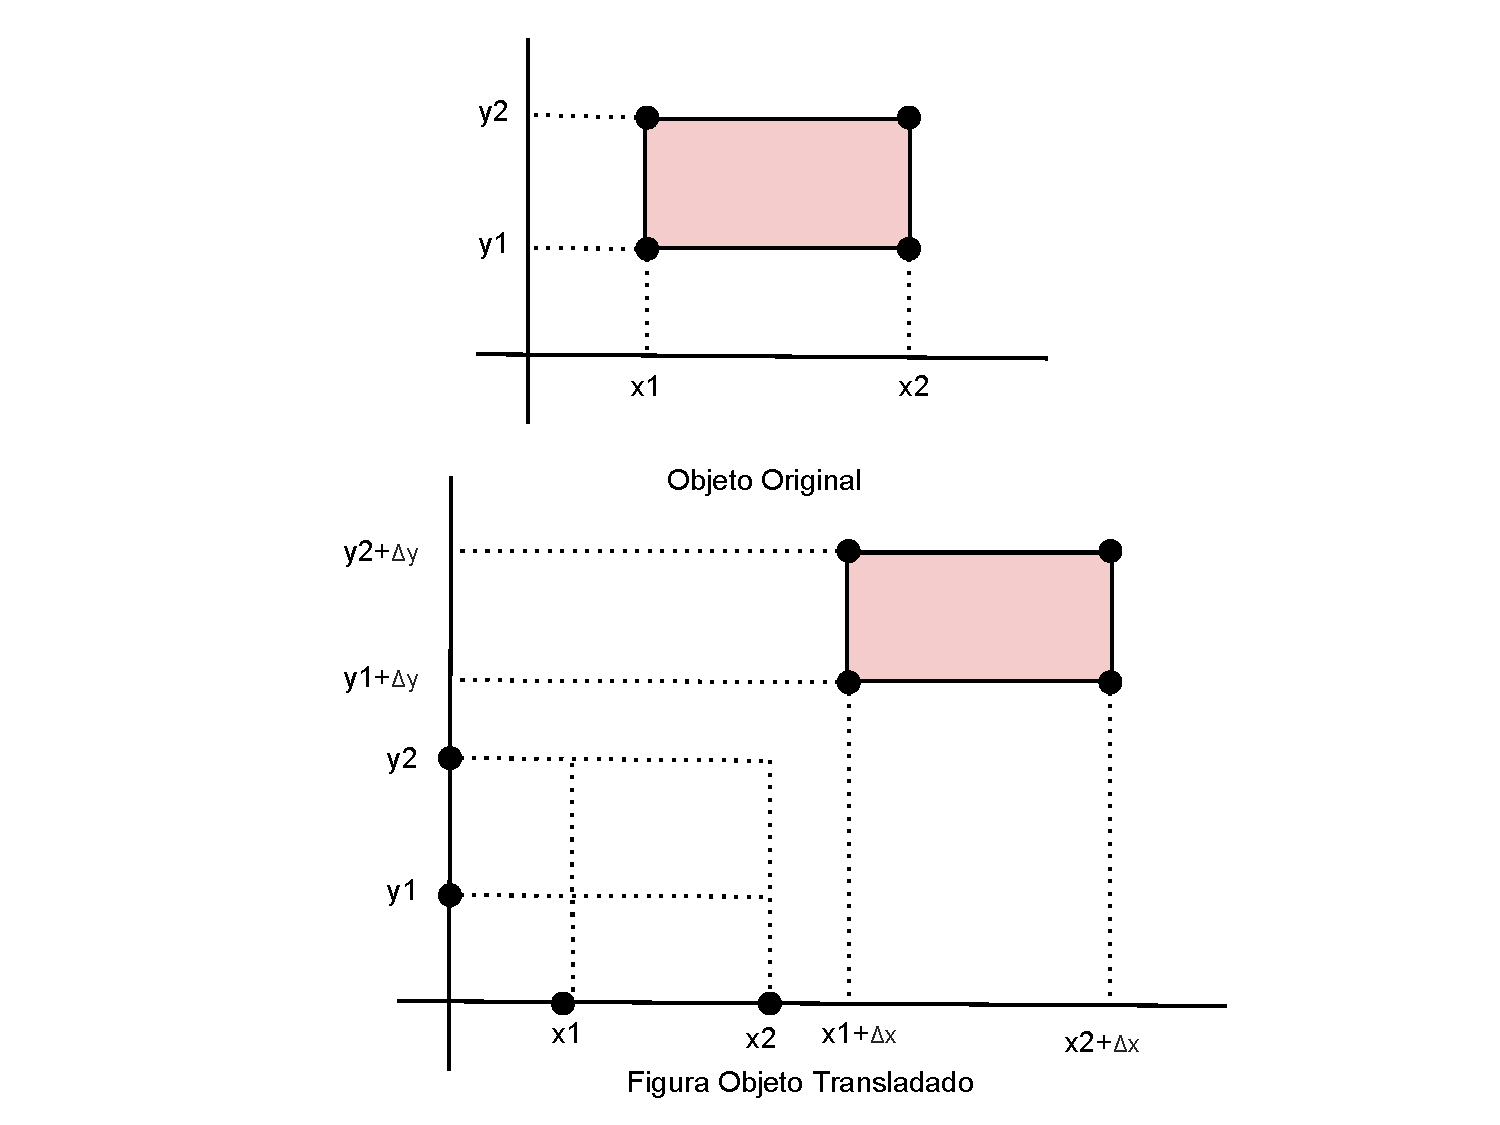
\includegraphics[width=0.9\textwidth]{Figures/Translacao}
			\end{center}
	\end{figure}	
	
\end{frame}

%%%%%%%%%%%%%%%%%%%%%%%%%%%%%%%%%%%%%%%%%%%%%%%%%%%%%%%%%%%%%%%%%%%%%%%%%%%%%%%%%%%%%%%%%%
\begin{frame}
\frametitle{Translação}


	\begin{block}{Translação de um Objeto}
		\begin{itemize}
			\item A translação consiste em adicionar uma ``variação'' as coordenadas de um objeto.
			\begin{itemize}
				\item $x' = x + \Delta x$
				\item $y' = y + \Delta y$
			\end{itemize}
		\end{itemize}
		
	\end{block}
	
	\begin{block}{Notação Matricial}
		\begin{itemize}
			\item Utilizando uma notação matricial é possível representar a operação de translação da seguinte forma:
		\end{itemize}
		\begin{eqnarray*}
			\textbf{P}' = \textbf{P} + \textbf{T} \\
			\textbf{P}' = 	\begin{bmatrix} 
								x' \\
								y' \\
							\end{bmatrix}
			,\textbf{P} = 	\begin{bmatrix}
								x \\
								y \\
							\end{bmatrix}
			,\textbf{T} = 	\begin{bmatrix}
								\Delta x \\
								\Delta y \\
							\end{bmatrix}
		\end{eqnarray*}
		
	\end{block}
	
\end{frame}

%%%%%%%%%%%%%%%%%%%%%%%%%%%%%%%%%%%%%%%%%%%%%%%%%%%%%%%%%%%%%%%%%%%%%%%%%%%%%%%%%%%%%%%%%%
\section{Rotação}
\begin{frame}
\frametitle{Rotação}


	\begin{block}{Rotação de um Objeto}
		\begin{itemize}
			\item Dá-se a operação de rotação de um objeto através de um \textbf{eixo de rotação} e um \textbf{ângulo de rotação}.
			\item No plano 2D, o eixo de rotação dá-se pelo eixo perpendicular ao plano $xy$.
		\end{itemize}
	\end{block}
	
	\begin{figure}[!h]
			\begin{center}
			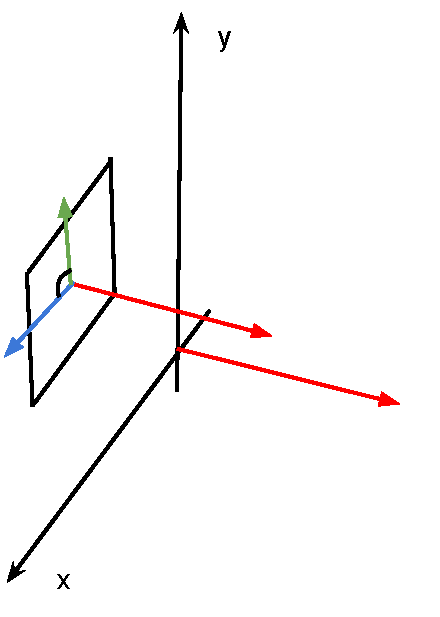
\includegraphics[width=0.3\textwidth]{Figures/EixoRotacao2D}
			\end{center}
	\end{figure}
	
\end{frame}

%%%%%%%%%%%%%%%%%%%%%%%%%%%%%%%%%%%%%%%%%%%%%%%%%%%%%%%%%%%%%%%%%%%%%%%%%%%%%%%%%%%%%%%%%%

\begin{frame}
\frametitle{Rotação}


	\begin{block}{Rotação de um Objeto}
		\begin{itemize}
			\item Para realizar a rotação de um objeto em 2D, é necessário um ângulo $\theta$ e o ponto de ponto de rotação $(x,y)$, que é o ponto de intersecção com o eixo perpendicular ao plano $xy$.
			\begin{itemize}
				\item Se $\theta > 0$, a rotação é no sentido anti-horária.
				\item Se $\theta < 0$, a rotação é no sentido horário.
			\end{itemize}
		\end{itemize}
	\end{block}
	
	\begin{figure}[!h]
			\begin{center}
			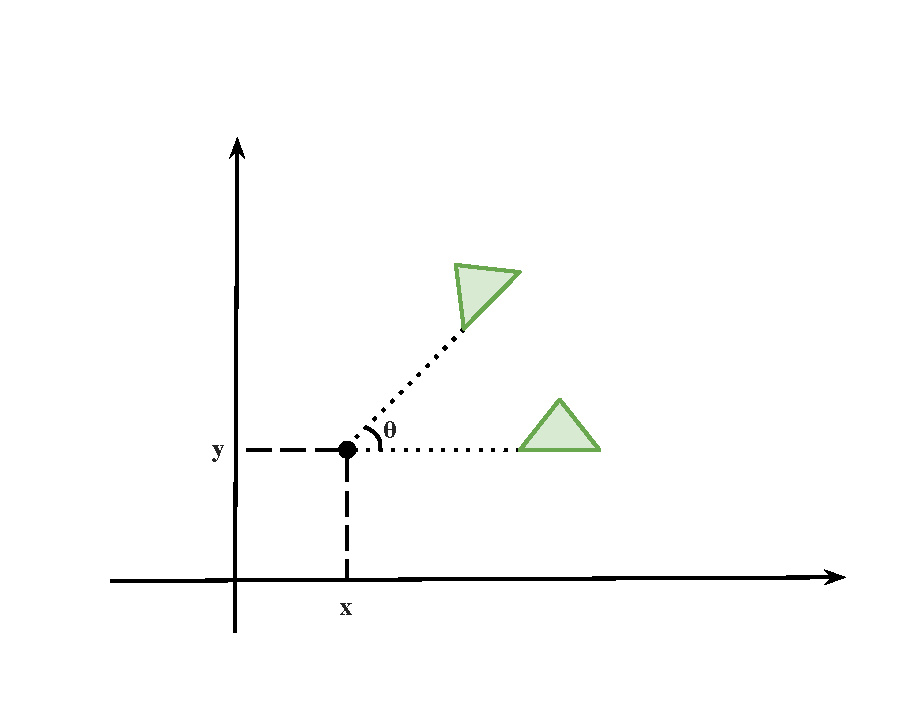
\includegraphics[width=0.5\textwidth]{Figures/ExemploRotacao}
			\end{center}
	\end{figure}
	
\end{frame}

%%%%%%%%%%%%%%%%%%%%%%%%%%%%%%%%%%%%%%%%%%%%%%%%%%%%%%%%%%%%%%%%%%%%%%%%%%%%%%%%%%%%%%%%%%

\begin{frame}
\frametitle{Rotação}


	\begin{block}{Rotação de um Objeto}
		\begin{itemize}
			\item Simplificando:
			\begin{itemize}
				\item Considera-se que o ponto de rotação está na origem.
				\item O raio $r$ é constante.
				\item $\phi$ é o ângulo do ponto $P = (x,y)$ em relação a origem.
				\item $\theta$ é o ângulo de rotação.
			\end{itemize}
		\end{itemize}
	\end{block}
	
	\begin{figure}[!h]
			\begin{center}
			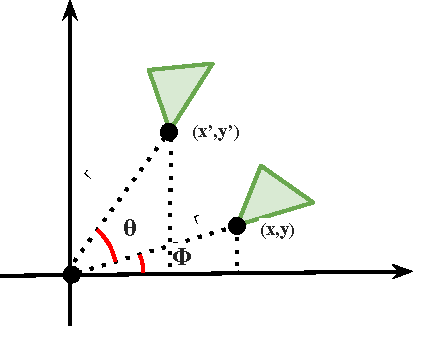
\includegraphics[width=0.5\textwidth]{Figures/ExemploRotacao2}
			\end{center}
	\end{figure}
	
\end{frame}

%%%%%%%%%%%%%%%%%%%%%%%%%%%%%%%%%%%%%%%%%%%%%%%%%%%%%%%%%%%%%%%%%%%%%%%%%%%%%%%%%%%%%%%%%%

\begin{frame}
\frametitle{Rotação}

	\begin{block}{Sabemos que:}
		\begin{itemize}
			\item $cos(\theta) = \frac{\text{Cateto adjacente}}{\text{Hipotenuza}}$
			\item $sen(\theta) = \frac{\text{Cateto oposto}}{\text{Hipotenuza}}$
		\end{itemize}
	\end{block}

	\begin{block}{Então temos que:}
		\begin{itemize}
			\item $cos(\phi + \theta) = \frac{x'}{r} \implies x' = cos(\phi + \theta)\cdot r$
			\item $sen(\phi + \theta) = \frac{y'}{r} \implies y' = sen(\phi + \theta)\cdot r$
		\end{itemize}
	\end{block}
	
\end{frame}


%%%%%%%%%%%%%%%%%%%%%%%%%%%%%%%%%%%%%%%%%%%%%%%%%%%%%%%%%%%%%%%%%%%%%%%%%%%%%%%%%%%%%%%%%%

\begin{frame}
\frametitle{Rotação}

	\begin{block}{Como:}
		\begin{itemize}
			\item $cos(\alpha + \beta) = cos(\alpha) \cdot cos(\beta) - sen(\alpha)\cdot sen(\beta)$
			\item $sen(\alpha + \beta) = cos(\alpha) \cdot sen(\beta)   + sen(\alpha)\cdot cos(\beta)$
		\end{itemize}
	\end{block}

	\begin{block}{Então temos que:}
		\begin{itemize}
			\item $ x' =  r \cdot cos(\phi) \cdot cos(\theta) - r \cdot sen(\phi) \cdot sen(\theta)$
			\item $ y' =  r \cdot cos(\phi) \cdot sen(\theta) + r \cdot sen(\phi) \cdot cos(\theta)$
		\end{itemize}
	\end{block}
	
\end{frame}

%%%%%%%%%%%%%%%%%%%%%%%%%%%%%%%%%%%%%%%%%%%%%%%%%%%%%%%%%%%%%%%%%%%%%%%%%%%%%%%%%%%%%%%%%%

\begin{frame}
\frametitle{Rotação}

	\begin{block}{Coordenadas Polares}
		\begin{itemize}
			\item<1-> Temos que $P = (x,y)$ pode ser escrito na forma de coordenadas polares:
				\begin{itemize}
					\item $x = r \cdot cos(\theta)$
					\item $y = r \cdot sen(\theta)$ 
				\end{itemize}
			\item<2-> Substituindo os valores temos:
				\begin{itemize}
					\item $x' = x \cdot cos(\theta) - y \cdot sen(\theta)$
					\item $y' = x \cdot sen(\theta) + y \cdot cos(\theta)$
				\end{itemize}
		\end{itemize}
	\end{block}
	
	\begin{block}{Em Notação de Matriz}
		\begin{eqnarray*}
			\textbf{P}' = \textbf{R} \cdot \textbf{P} \\
			\textbf{P}' = 	\begin{bmatrix} 
								x' \\
								y' \\
							\end{bmatrix}
			=
			 \begin{bmatrix}
								cos(\theta) & -sen(\theta) \\
								sen(\theta) & cos(\theta)\\
							\end{bmatrix}
			\cdot \begin{bmatrix}
								x \\
								y \\
							\end{bmatrix}
		\end{eqnarray*}
	\end{block}

	
\end{frame}


%%%%%%%%%%%%%%%%%%%%%%%%%%%%%%%%%%%%%%%%%%%%%%%%%%%%%%%%%%%%%%%%%%%%%%%%%%%%%%%%%%%%%%%%%%

\begin{frame}
\frametitle{Rotação}


	\begin{block}{Rotação de em Torno de um Ponto Arbitrário}
			\begin{itemize}
				\item Rotação em torno de um ponto $(x_r,y_r)$.
			\end{itemize}
	\end{block}
	
	\begin{figure}[!h]
			\begin{center}
			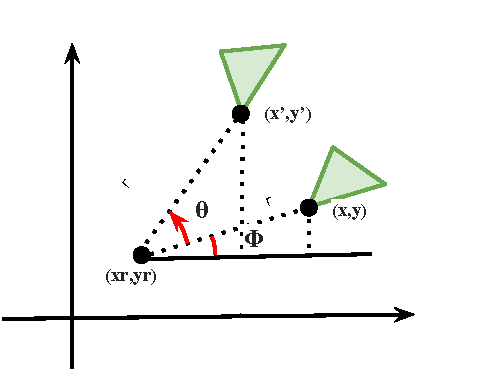
\includegraphics[width=0.5\textwidth]{Figures/ExemploRotacao3}
			\end{center}
	\end{figure}
	
	
	
\end{frame}

%%%%%%%%%%%%%%%%%%%%%%%%%%%%%%%%%%%%%%%%%%%%%%%%%%%%%%%%%%%%%%%%%%%%%%%%%%%%%%%%%%%%%%%%%%

\begin{frame}
\frametitle{Rotação}

	\begin{block}{Para encontrar $x'$}
		\begin{itemize}
			\item $cos (\phi + \theta) = \frac{x' - x_r}{r}$
			\item $x' = r \cdot cos (\phi + \theta) + x_r $	
			\item $x' = x_r + r \cdot cos(\phi) \cdot cos (\theta) - r \cdot sen(\phi) \cdot sen(\theta)$
		\end{itemize}
	\end{block}
	
	\begin{block}{Mas temos que:}
		\begin{itemize}
			\item $cos (\phi) = \frac{x-x_r}{r}$ e $sen(\phi) =\frac{y - y_r}{r}$ 
		\end{itemize}
	\end{block}
	
	\begin{block}{Então:}
		\begin{itemize}
			\item $x' = x_r + (x - x_r) \cdot cos(\theta) - (y-y_r) \cdot sen(\theta)$
			\item $y' = y_r + (x - x_r) \cdot sen(\theta) + (y-y_r) \cdot cos(\theta)$ 
		\end{itemize}
	\end{block}
	
\end{frame}


%----------------------------------------------------------------------------------------

\end{document} 